% SC4053 --- Chapter 2: Consensus (PoW, PoS, BFT) (0->100)
\chapter{Consensus: Proof-of-Work, Proof-of-Stake and BFT}\label{ch:consensus}

\begin{quote}
\emph{``Consensus is how strangers agree on one history when anyone can propose the next page.''} --- From mining puzzles to validator lotteries to Byzantine voting, this chapter derives why agreement is hard and how blockchains achieve it.
\end{quote}

\noindent\fbox{\parbox{\dimexpr\linewidth-2\fboxsep-2\fboxrule}{%
\textbf{From zero: no consensus background assumed.} We start from a classroom where every student shouts a different answer - how do you pick one? We build intuition with lotteries, then formalise safety/liveness/finality, and compare PoW, PoS and BFT step by step with runnable lotteries.}}
\vspace{0.4em}

\section*{Learning Outcomes}
After this chapter you will be able to:
\begin{enumerate}[label=(L\arabic*)]
    \item state safety, liveness and finality for a blockchain and why FLP matters;
    \item derive PoW success probability, difficulty adjustment and expected block time;
    \item explain PoS selection, slashing and the nothing-at-stake problem;
    \item trace PBFT's three phases and the $n\ge 3f+1$ bound;
    \item compare PoW/PoS/BFT on energy, throughput and adversary thresholds.
\end{enumerate}

% ============================================================
\section{The Consensus Problem}\label{sec:consensus-problem}
A blockchain is a replicated log: every honest node should eventually hold the same sequence $B_0,B_1,\dots$. In SC4051 terms this is total-order broadcast, but now participants are \emph{open} (anyone can join) and \emph{Byzantine} (some may lie for profit). Classical consensus assumed a fixed $n$; blockchain consensus must work with unknown, changing $n$ and economic incentives.

\begin{definition}[Safety, liveness, finality]\label{def:safety-live}
\emph{Safety}: no two honest nodes commit different blocks at the same height. \emph{Liveness}: new honest transactions are eventually committed. \emph{Finality} is the guarantee that a committed block will never be reverted -- \emph{probabilistic} (reversion probability decays with depth, as in Bitcoin) vs \emph{deterministic} (once committed, never reverted, as in PBFT).
\end{definition}

The FLP impossibility (Fischer--Lynch--Paterson) says deterministic consensus is impossible in fully asynchronous networks with one crash. Blockchains escape FLP by adding randomness (PoW lottery), timing assumptions (partial synchrony for BFT), or economic stakes (PoS).

% ============================================================
\section{Proof-of-Work: The Mining Lottery}\label{sec:pow}
PoW turns block proposal into a computational lottery. To propose $B_i$, a miner repeatedly picks a nonce $n$ and checks
\begin{equation}\label{eq:pow}
H(\text{header}(B_i)\parallel n) < T,\quad T = \frac{2^{256}}{D},
\end{equation}
where $D$ is \emph{difficulty}. The smaller $T$, the harder the puzzle. Because $H$ is pseudorandom, each try succeeds with probability $p=T/2^{256}=1/D$, independent of history.

\begin{figure}[h]\centering
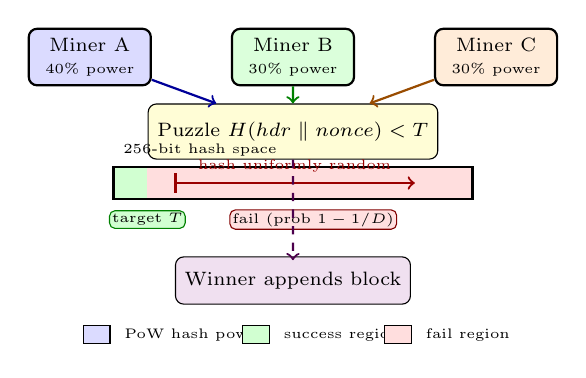
\begin{tikzpicture}[scale=0.86, every node/.style={font=\scriptsize},
  miner/.style={draw,rounded corners=3pt,minimum width=1.55cm,minimum height=0.65cm,align=center,thick}]
\node[miner,fill=blue!14] (m1) at (0,2.00) {Miner A\\ \tiny 40\% power};
\node[miner,fill=green!14] (m2) at (3.0,2.00) {Miner B\\ \tiny 30\% power};
\node[miner,fill=orange!15] (m3) at (6.0,2.00) {Miner C\\ \tiny 30\% power};
\node[draw,fill=yellow!16,rounded corners=3pt,minimum width=2.6cm,minimum height=0.70cm,align=center] (puz) at (3.0,0.90) {Puzzle $H(hdr\parallel nonce)<T$};
\draw[->,thick,blue!60!black] (m1)--(puz); \draw[->,thick,green!50!black] (m2)--(puz); \draw[->,thick,orange!60!black] (m3)--(puz);
% target bar
\fill[red!13] (0.35,-0.10) rectangle (5.65,0.38);
\fill[green!18] (0.35,-0.10) rectangle (0.85,0.38);
\draw[thick] (0.35,-0.10) rectangle (5.65,0.38);
\node[font=\tiny,anchor=west] at (0.35,0.62) {256-bit hash space};
\node[font=\tiny,fill=green!18,draw=green!50!black,rounded corners=2pt,inner sep=1pt] at (0.85,-0.40) {target $T$};
\node[font=\tiny,fill=red!12,draw=red!50!black,rounded corners=2pt,inner sep=1pt] at (3.30,-0.40) {fail (prob $1-1/D$)};
\draw[|->,thick,red!60!black] (1.25,0.14) -- (4.80,0.14) node[midway,above,font=\tiny] {hash uniformly random};
% chain tip
\node[draw,fill=violet!12,rounded corners=3pt,minimum width=2.2cm,minimum height=0.60cm,align=center] at (3.0,-1.30) {Winner appends block};
\draw[->,thick,violet!60!black,dashed] (puz)--(3.0,-1.00);
% legend
\node[draw,fill=blue!14,minimum width=0.34cm,minimum height=0.20cm] at (0.10,-2.10) {}; \node[font=\tiny,anchor=west] at (0.37,-2.10) {PoW hash power};
\node[draw,fill=green!18,minimum width=0.34cm,minimum height=0.20cm] at (2.45,-2.10) {}; \node[font=\tiny,anchor=west] at (2.72,-2.10) {success region};
\node[draw,fill=red!13,minimum width=0.34cm,minimum height=0.20cm] at (4.55,-2.10) {}; \node[font=\tiny,anchor=west] at (4.82,-2.10) {fail region};
\end{tikzpicture}
\caption{PoW as a parallel lottery: each hash is an independent ticket, uniform in $[0,2^{256})$. Success lands in the tiny green target $T$; difficulty $D$ sets $T=2^{256}/D$. Whoever hits $T$ first wins the block.}
\label{fig:pow-lottery}
\end{figure}

If the global hash rate is $r$ hashes/s, the network finds a block as a Poisson process with rate $\lambda=r/D$, so expected block time $\mathbf{E}[T_{\text{block}}]=D/r$. Bitcoin retargets $D$ every 2016 blocks to keep $\mathbf{E}[T_{\text{block}}]\approx10$ min.

\begin{lstlisting}[language=Python]
import hashlib, time, random
def sha256d(b): return hashlib.sha256(hashlib.sha256(b).digest()).hexdigest()
def mine(header_prefix, target_hex, max_nonce=5000000):
    T = int(target_hex, 16)
    for nonce in range(max_nonce):
        h = hashlib.sha256((header_prefix+str(nonce)).encode()).hexdigest()
        if int(h,16) < T:
            return nonce, h
    return None
# Demo: difficulty with 3 leading hex zeros (12 bits)
target = "000"+"f"*61          # ~ D = 16^3 = 4096
nonce, h = mine("block42|prev=abc|merkle=def|", target)
print(f"found nonce {nonce} hash {h[:16]}... < target")
# Expected tries ~ D = 4096, ~ milliseconds on a laptop; real Bitcoin D ~ 10^13x larger
\end{lstlisting}

\begin{remark}[Energy and incentives]\label{rem:energy}
PoW ties security to energy: rewriting $k$ blocks costs $\approx k\cdot D$ hashes. An attacker with $<50\%$ power succeeds with probability that decays exponentially in $k$ (Nakamoto's analysis). The cost is electricity; the reward is block subsidy plus fees. When reward $<$ cost, miners leave and security drops -- a coupling PoS tries to break.
\end{remark}

% ============================================================
\section{Proof-of-Stake: Lottery by Stake}\label{sec:pos}
PoS replaces energy with escrowed capital. Validators lock (\emph{stake}) coins; the protocol pseudo-randomly picks the next proposer with probability proportional to stake. No hashing race -- a single hash plus signature suffices.

\begin{figure}[h]\centering
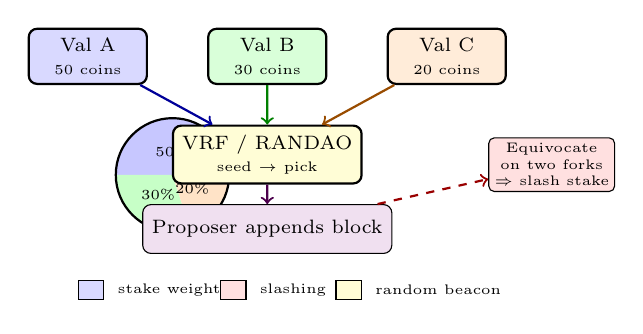
\begin{tikzpicture}[scale=0.86, every node/.style={font=\scriptsize},
  val/.style={draw,rounded corners=3pt,minimum width=1.50cm,minimum height=0.70cm,align=center,thick}]
\node[val,fill=blue!15] (v1) at (0,1.80) {Val A\\ \tiny 50 coins};
\node[val,fill=green!15] (v2) at (2.65,1.80) {Val B\\ \tiny 30 coins};
\node[val,fill=orange!15] (v3) at (5.30,1.80) {Val C\\ \tiny 20 coins};
% pie
\begin{scope}[xshift=1.25cm,yshift=0.05cm,scale=0.62]
  \fill[blue!22] (0,0) -- (0:1.35) arc (0:180:1.35) -- cycle;
  \fill[green!22] (0,0) -- (180:1.35) arc (180:288:1.35) -- cycle;
  \fill[orange!22] (0,0) -- (288:1.35) arc (288:360:1.35) -- cycle;
  \draw[thick] (0,0) circle (1.35);
  \node[font=\tiny] at (90:0.55) {50\%}; \node[font=\tiny] at (234:0.58) {30\%}; \node[font=\tiny] at (324:0.58) {20\%};
\end{scope}
\node[val,fill=yellow!16] (rnd) at (2.65,0.35) {VRF / RANDAO\\ \tiny seed $\to$ pick};
\draw[->,thick,blue!60!black] (v1)--(rnd); \draw[->,thick,green!50!black] (v2)--(rnd); \draw[->,thick,orange!60!black] (v3)--(rnd);
\node[draw,fill=violet!12,rounded corners=3pt,minimum width=2.45cm,minimum height=0.62cm,align=center] (win) at (2.65,-0.75) {Proposer appends block};
\draw[->,thick,violet!60!black] (rnd)--(win);
\node[draw,fill=red!12,rounded corners=2pt,inner sep=2pt,font=\tiny,align=center] (slash) at (6.85,0.20) {Equivocate\\on two forks\\$\Rightarrow$ slash stake};
\draw[->,thick,red!60!black,dashed] (win) -- (slash);
% legend
\node[draw,fill=blue!15,minimum width=0.32cm,minimum height=0.18cm] at (0.05,-1.65) {}; \node[font=\tiny,anchor=west] at (0.30,-1.65) {stake weight};
\node[draw,fill=red!12,minimum width=0.32cm,minimum height=0.18cm] at (2.15,-1.65) {}; \node[font=\tiny,anchor=west] at (2.40,-1.65) {slashing};
\node[draw,fill=yellow!16,minimum width=0.32cm,minimum height=0.18cm] at (3.85,-1.65) {}; \node[font=\tiny,anchor=west] at (4.10,-1.65) {random beacon};
\end{tikzpicture}
\caption{PoS proposer lottery weighted by stake, plus slashing (red) that punishes double-signing. Comparison: PoW weighs by hash power; PoS weighs by escrowed coins. Legend distinguishes power, randomness and punishment.}
\label{fig:pos-lottery}
\end{figure}

The \emph{nothing-at-stake} worry: without cost to vote on multiple forks, validators might rationally double-sign. Modern PoS (Ethereum's Gasper) adds \emph{slashing} (burn stake if you sign conflicting blocks), \emph{finality gadgets} (Casper FFG) and \emph{weak subjectivity} checkpoints so late joiners know the canonical chain.

\begin{lstlisting}[language=Python]
import random, hashlib
def pos_lottery(stakes, seed="beacon42"):
    # stakes: dict name -> coins; returns winner
    h = int(hashlib.sha256(seed.encode()).hexdigest(), 16)
    total = sum(stakes.values())
    pick = h % total
    cur = 0
    for name, s in stakes.items():
        cur += s
        if pick < cur: return name
stakes = {"Alice":50, "Bob":30, "Carol":20}
for seed in ["b0","b1","b2","b3","b4"]:
    print(seed, "->", pos_lottery(stakes, seed))
# Over many beacons, win rate -> 50/30/20%
\end{lstlisting}

% ============================================================
\section{Byzantine Fault Tolerance (BFT)}\label{sec:bft}
When the validator set is known and small ($n\approx100$), classical BFT shines. PBFT (Castro--Liskov) achieves deterministic finality with $n\ge 3f+1$ under partial synchrony.

\begin{figure}[h]\centering
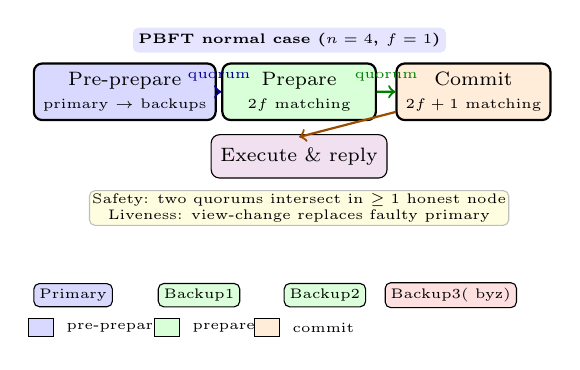
\begin{tikzpicture}[scale=0.82, every node/.style={font=\scriptsize},
  phase/.style={draw,rounded corners=3pt,minimum width=1.95cm,minimum height=0.60cm,align=center,thick}]
\node[font=\tiny\bfseries,fill=blue!10,rounded corners=2pt,inner sep=2pt] at (3.90,3.05) {PBFT normal case ($n=4$, $f=1$)};
\node[phase,fill=blue!15] (pre) at (1.35,2.25) {Pre-prepare\\ \tiny primary $\to$ backups};
\node[phase,fill=green!15] (prep) at (4.05,2.25) {Prepare\\ \tiny $2f$ matching};
\node[phase,fill=orange!15] (com) at (6.75,2.25) {Commit\\ \tiny $2f+1$ matching};
\draw[->,thick,blue!60!black] (pre)--(prep) node[midway,above,font=\tiny] {quorum};
\draw[->,thick,green!50!black] (prep)--(com) node[midway,above,font=\tiny] {quorum};
\node[draw,fill=violet!12,rounded corners=3pt,minimum width=2.15cm,minimum height=0.55cm,align=center] (exe) at (4.05,1.25) {Execute \& reply};
\draw[->,thick,orange!60!black] (com) -- (4.05,1.55);
% message counts
\node[font=\tiny,fill=yellow!12,draw=gray!50,rounded corners=2pt,inner sep=1pt,align=center] at (4.05,0.45) {Safety: two quorums intersect in $\ge1$ honest node\\Liveness: view-change replaces faulty primary};
% participants lane
\begin{scope}[yshift=-0.35cm]
  \foreach \i/\lab/\col in {0/Primary/blue!15,1/Backup1/green!14,2/Backup2/green!14,3/Backup3( byz)/red!12} {
    \node[font=\tiny,fill=\col,draw,rounded corners=2pt,inner sep=2pt] at (\i*1.95+0.55,-0.55) {\lab};}
\end{scope}
% legend
\node[draw,fill=blue!15,minimum width=0.32cm,minimum height=0.18cm] at (0.05,-1.40) {}; \node[font=\tiny,anchor=west] at (0.30,-1.40) {pre-prepare};
\node[draw,fill=green!15,minimum width=0.32cm,minimum height=0.18cm] at (2.00,-1.40) {}; \node[font=\tiny,anchor=west] at (2.25,-1.40) {prepare};
\node[draw,fill=orange!15,minimum width=0.32cm,minimum height=0.18cm] at (3.55,-1.40) {}; \node[font=\tiny,anchor=west] at (3.80,-1.40) {commit};
\end{tikzpicture}
\caption{PBFT's three-phase commit with quorum intersections. Each phase needs $2f+1$ matching messages, guaranteeing any two quorums share an honest node -- the source of the $3f+1$ bound. Liveness comes from view-change timeouts.}
\label{fig:pbft}
\end{figure}

\begin{theorem}[BFT lower bound]\label{thm:bft-bound}
No deterministic BFT protocol tolerates $f$ Byzantine faults with $n\le 3f$ in partial synchrony.
\end{theorem}
\emph{Sketch.} Partition $n=3f$ into three groups $A,B,C$ of $f$ each. Byzantine $C$ can mimic $A$ to $B$ and $B$ to $A$, making $A$ and $B$ decide differently while each sees a quorum of $2f$. \hfill$\square$

In practice, Tendermint/Cosmos and HotStuff (used in later BFT chains) streamline PBFT's view-change with a rotating leader and linear communication.

\begin{example}[Choosing a consensus]\label{ex:choose}
A permissionless currency wants open entry and 10\,min blocks: PoW or PoS fits. A supply-chain consortium with 20 known firms wanting 1\,s finality: PBFT/Tendermint fits -- faster, deterministic, but closed membership. Many modern chains hybridise: PoS for Sybil resistance plus a BFT finality gadget.
\end{example}

% ============================================================
\section{Difficulty Adjustment and Fork Choice}\label{sec:fork-choice}
Difficulty does not stay fixed. Bitcoin adjusts every 2016 blocks: $D_{\text{new}}=D_{\text{old}}\cdot (2016\cdot600)/T_{\text{actual}}$ where $T_{\text{actual}}$ is the time the last 2016 blocks took. If blocks came too fast ($T_{\text{actual}}<2016\cdot600$), $D$ rises; too slow, $D$ falls. This negative feedback keeps block time near 10\,min despite hash-rate swings.

Fork choice: when two blocks appear at the same height, honest nodes follow the \emph{heaviest chain} (most accumulated work, which for equal $D$ is the longest). An attacker who withholds blocks creates a hidden fork; releasing it can reorg the honest chain if it is heavier. PoS fork choice (LMD-GHOST plus Casper FFG) weighs attestations rather than work, but the heaviest-observed-subtree idea is analogous: the fork with most validator votes wins, and finalised checkpoints cannot be reverted without slashing.

\begin{example}[Retarget arithmetic]\label{ex:retarget}
Suppose last 2016 blocks took 12 days instead of 14. Then $D_{\text{new}}=D_{\text{old}}\cdot 14/12\approx1.17\,D_{\text{old}}$: difficulty rises 17\% to slow blocks back to 10\,min. Halving hash rate has the opposite effect.
\end{example}

\begin{remark}[Why 10\,min?]\label{rem:tenmin}
Shorter block time reduces confirmation latency but raises fork rate (more simultaneous proposers due to propagation delay). Bitcoin's 10\,min is a compromise: propagation ($\sim$1--10\,s) $\ll$ block time, so forks are rare ($<1\%$). Ethereum targets $\sim$12\,s because GHOST/uncle rules tolerate more forks.
\end{remark}

% ============================================================
\section{Exercises}\label{sec:ch02-exercises}
\begin{enumerate}[label=E2.\arabic*, leftmargin=*, itemsep=0.6em]
    \item \textbf{Block-time math.} Global hash rate $r=200$ EH/s, difficulty $D=6\times10^{13}$. Compute expected block time $D/r$ and success probability per hash. If $D$ doubles, what retarget keeps 10\,min?
    \item \textbf{PoW vs PoS cost.} An attacker rents 51\% hash for 6 blocks vs bribes 51\% stake with slashing risk. Model both costs with numbers and argue which is more ``expensive to repeat.''
    \item \textbf{PBFT trace.} With $n=7$, $f=2$, how many Prepare and Commit messages does an honest replica collect before proceeding? Show why $n=6$ fails the intersection argument.
    \item \textbf{Selfish mining.} A miner with 30\% power withholds a found block. Sketch when releasing it causes a fork and when honest miners waste work. What threshold makes selfish mining profitable?
    \item \textbf{Finality comparison.} A merchant accepts 0-conf vs 6-conf on PoW vs single-slot finality on PBFT. Assign reversion probabilities and justify your confirmation policy for a 10\,k payment.
\end{enumerate}

\section*{Chapter Notes}
Nakamoto (2008) for PoW; Buterin's Casper and the Ethereum PoS specs (2020-22) for PoS/slashing; Castro--Liskov, ``Practical BFT'' (OSDI 1999) for PBFT; Dwork--Lynch--Stockmeyer (1988) for partial synchrony; Yin et al., HotStuff (PODC 2019) for linear BFT. Narayanan et al., Ch.~2-3 is the best first-principles companion.
% End Ch02
